In this section the different tasks that Beaglebone has o perform are described in detail. In this project the \textit{Linux distro} used is \textit{Debian}. It has been chosen among the wide possibilities because ensure a good level of stability, and moreover it has a very good repository. 

\begin{figure}[h]
	\centering
	\begin{tikzpicture}[
	level 1/.style={sibling distance=40mm},
	edge from parent/.style={->,draw, black},
	>=latex, scale=0.75, every node/.style={scale=0.70}]
	
	% root of the the initial tree, level 1
	\node[root] {Embedded Linux Firmware}
	% The first level, as children of the initial tree
	child {node[level 2] (c1) {Video Acquisition}
		child{node[level 3] {Beating Plot Computation}}
		%child{node[level 3] {Electrovalves Driver}}
		%child{node[level 3] {Power Supply}}
		}
	child {node[level 2] (c2) {Sensors Data Acquisition}}
	child {node[level 2] (c3) {Electrovalves Driver}
		};

	
	\end{tikzpicture}
	\caption{Embedded Linux Firmware - Blocks Subdivision}
	\label{Fig:firmware}
\end{figure}

In (Fig.\ref{Fig:firmware}) are shown the three principle subsection of the firmware. For each of them a \textit{C++} program has been written, and their executable files are going to be run through a \textit{bash} script, which is supposed to be launched at the system boot. The (List.\ref{code:recordVideo}) shown this bash script that behaves as shown in (Fig.\ref{Fig:bash}).

First of all the \textit{bash} script loads the \textit{Device Tree Overlay}. The pins of \textit{Sitara\texttrademark} microprocessor are \textit{multiplexed}, it means that each pin of the two header may assume different behavior (\textit{GPIO}, \textit{SPI}, \textit{I2C}, and so on..). During the booting a default value for this mux is loaded, and for certain pins, this default value differs from the actual value that the system needs. In order to change those values I wrote a Device Tree Overlays (\textit{DTO}) which has to run at the beginning, immediately after the booting, in order to explain how is it work the Flattened Device Tree (\textit{FDT}) has to be introduced.

The last releases of Linux kernels for ARM boards use \textit{FDT}, it is a data structure that describes the hardware on board. Thus, it describes every component presents on the board, from the user \textit{LEDs} to the \textit{CPU}. Using this \textit{FDT} it is possible to write a \textit{device tree overlay} in order to change to mode of use of each pin. The (List.\ref{code:pins}) changes the status of $10$ pins from their default value, in particular sets the pins used to drive the valves, to allow the current on resistor sensor, and to change the power supply voltage on the valves to be digital output pins, with a pulldown resistor.

To record the video from the microscope I used the program \textit{\textbf{Video for Linux v.2}} (\textit{V4L2}), before start record the \textit{bash} script sets the video format as \textit{MJPG} and the dimension as $320\ x\ 240\ @ 30\ fps$. After that it runs in background the program to update the electrovalves status and to acquire the sensors value. As it is explained in (Sec.\ref{sec:valves}), these programs run out of the infinite loop because they have an infinite loop inside.

Inside the infinite loop the \textit{bash} script launch the recording of $10$ seconds microscope video, compresses the latter and elaborate it in order to compute an image with the beating plot. Finally, it uploads (using the library \textit{CURL}) video and image and update the flags that in order to indicate to Google Glass App and Video Storing software that a new video has been updated.

\begin{figure}[h]
	\centering
	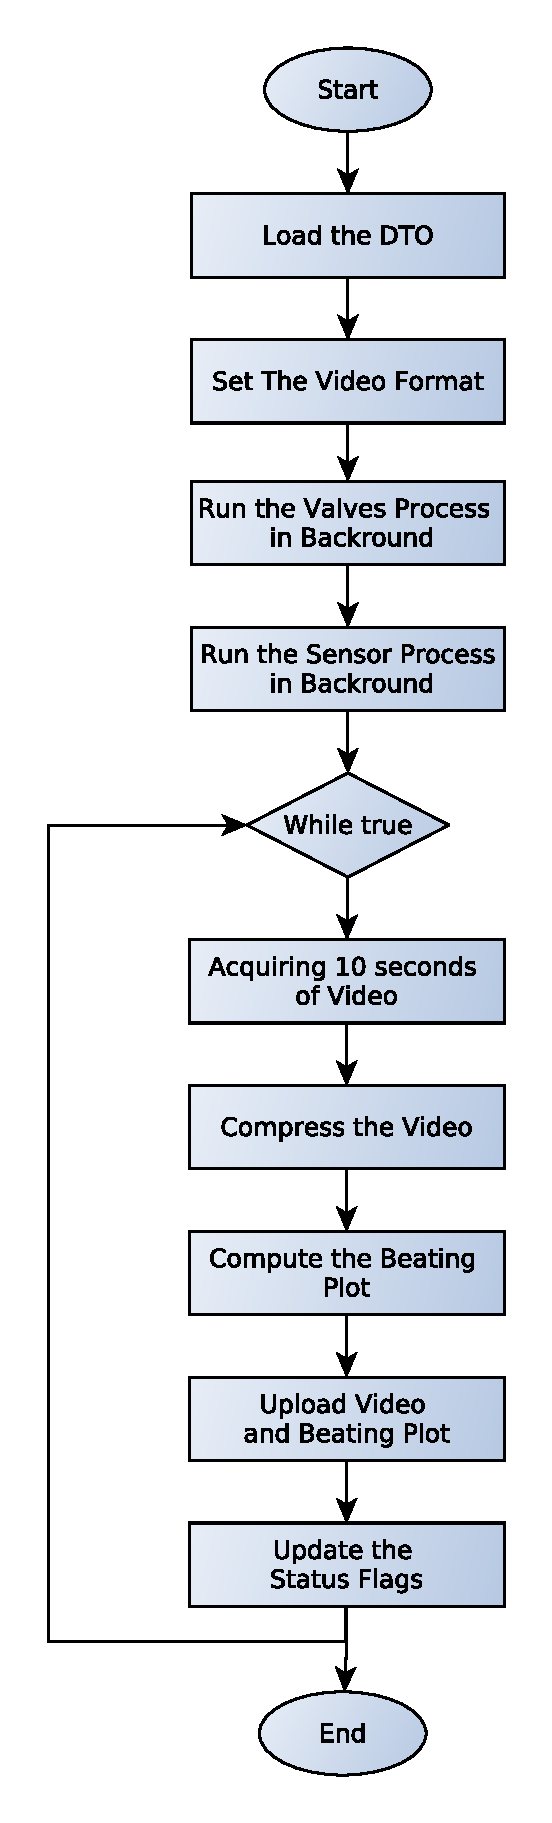
\includegraphics[height = .74\textheight]{firmware/bash}
	\caption{Bash Script Flow Chart}
	\label{Fig:bash}
	
\end{figure}
\clearpage

\section{Video Processing and Beating Plot}

As already introduced once the microscope video has been recorded in a \textit{MP4} format it has to be processed in order to compute the beating rate. The code described in this section is shown in (List.\ref{code:beating}). 

To achieve this goal, the \textit{OpenCV} library has been used. It is a specific library for computer vision.

As can be seen the program captures the video from the file and, elaborating frame by frame it computes the point to be plotted. In particular it sores the first frame of video, then each point is given by the mean different color density between the under study frame and the first one.

The results has been stored in file called \textit{video\_data.dat}. This file is going to be the input for the \textit{gnuplot} task that is in charge to plot the beating data.

\section{Sensor Data Acquisition}

From the main \textit{bash} script another one is launched for acquiring the sensors data. This script is shown in (list.\ref{code:sensorbash}) and as can be seen it is an infinite loop where two operations are performed:
\begin{enumerate}
	\item cleaning the previous data from the datastore of Google App Engine server, otherwise plots on the Google Glass are impossible to be viewed;
	\item acquiring and uploading $100$ new sensors data. 
\end{enumerate} 

This second step is performed by another task shown in (List.\ref{code:sensors}), in which three objects have been used (Fig.\ref{Fig:umlsensors}). 

How it works: using a for loop, program runs $100$ times the reading of pH and temperature values, after that the reading step has been accomplished, the program is in charge to store these value on the Datastore of Google App Engine then it waits for $100\ ms$. Two important features has to be highlighted:
\begin{enumerate}
	\item as already introduced in (Sec.\ref{tempcon}), there is a \textit{BJT} inside the temperature conditioning circuit that acts as software-controlled switch. This is necessary to avoid the self-heating of temperature sensor and ensure a correct measure. This software-controlling may be seen from the code, indeed there is a digital output called \textit{temperature\_disable} that is normally denied, and it is asserted only when a temperature measure has to be carried out;
	\item as already introduced in (Sec.\ref{phcon}), the pH measuring process need to know exactly how much is the amount of added offset. Indeed, in order to make the pH sensor response unipolar, the circuit polarizes the negative pin of pH sensor at approximately $512\ mV$. Instead of using the theoretical value it is better to measure it just before every pH measure process. This is easily viewable from the code. 
\end{enumerate}   

\begin{figure}[h]
	\centering
	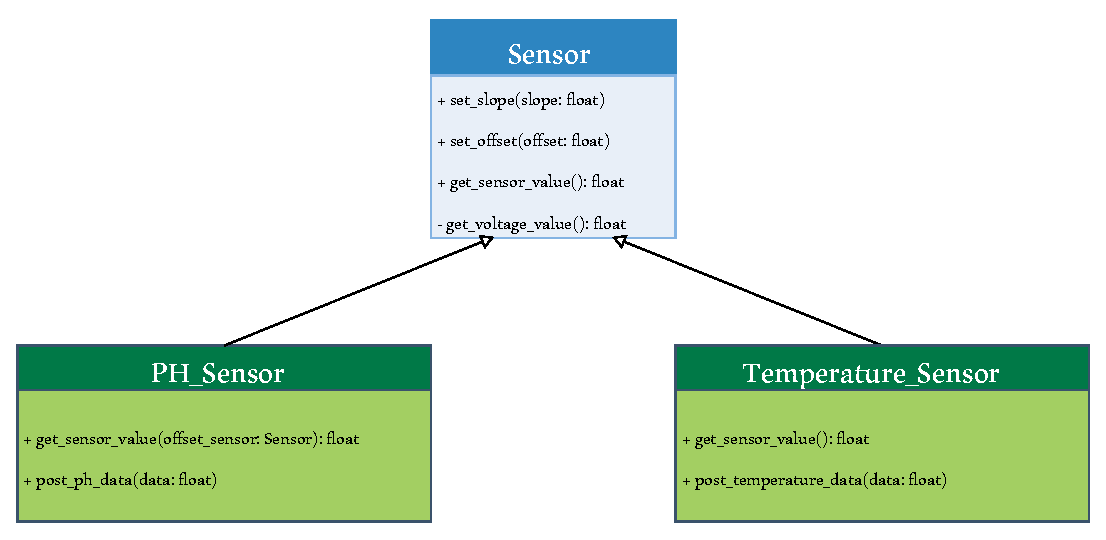
\includegraphics[width = \textwidth]{Sensors/class}
	\caption{Sensor UML Description}
	\label{Fig:umlsensors}
	
\end{figure}

\section{Electrovalves Updating Task}\label{sec:valves}

The code of task which performs the driving of the valves is shown in (List.\ref{code:Electrovalves}). Also this program uses the \textit{curl} library to communicate with the Google App Engine, and also this program has been built with an infinite loop.

What the task does is to download from the Google App Engine the status of each electrovalve that has been set by the user through the Google Glass. These status value are then stored onto a vector, to be written in a second step onto the output pins. As explained in (Sec.\ref{sec:electrovalves}) each valve is connected to a \textit{MOS} transistor that acts as voltage-controlled switch. The voltage which drives the transistor is the digital value written onto the output pins.

The task may be called with a parameter, the suply voltage value for valves:
\begin{verbatim}
./ValvesUpdating [12 | 24]
\end{verbatim}
If the parameter is missing, $24\ V$ as voltage are assumed as default. This parameter is going to drive both the \textit{DC-DC} enable and relay selector. In fact, if the voltage is the default one, the \textit{DC-DC} does not need to work, and so, in order to reduce the power consumption, be disabled.
\cleardoublepage